%************************************************
\chapter{Crystallization}
%************************************************
\begin{flushright}
March 18, 2013
\end{flushright}
\section{Aim}
To separate Napthalene from a mixture of it with Aniline, using the crystallization technique

\section {Chemicals Required}
	\begin{figure}[bth]
		\begin{center}
			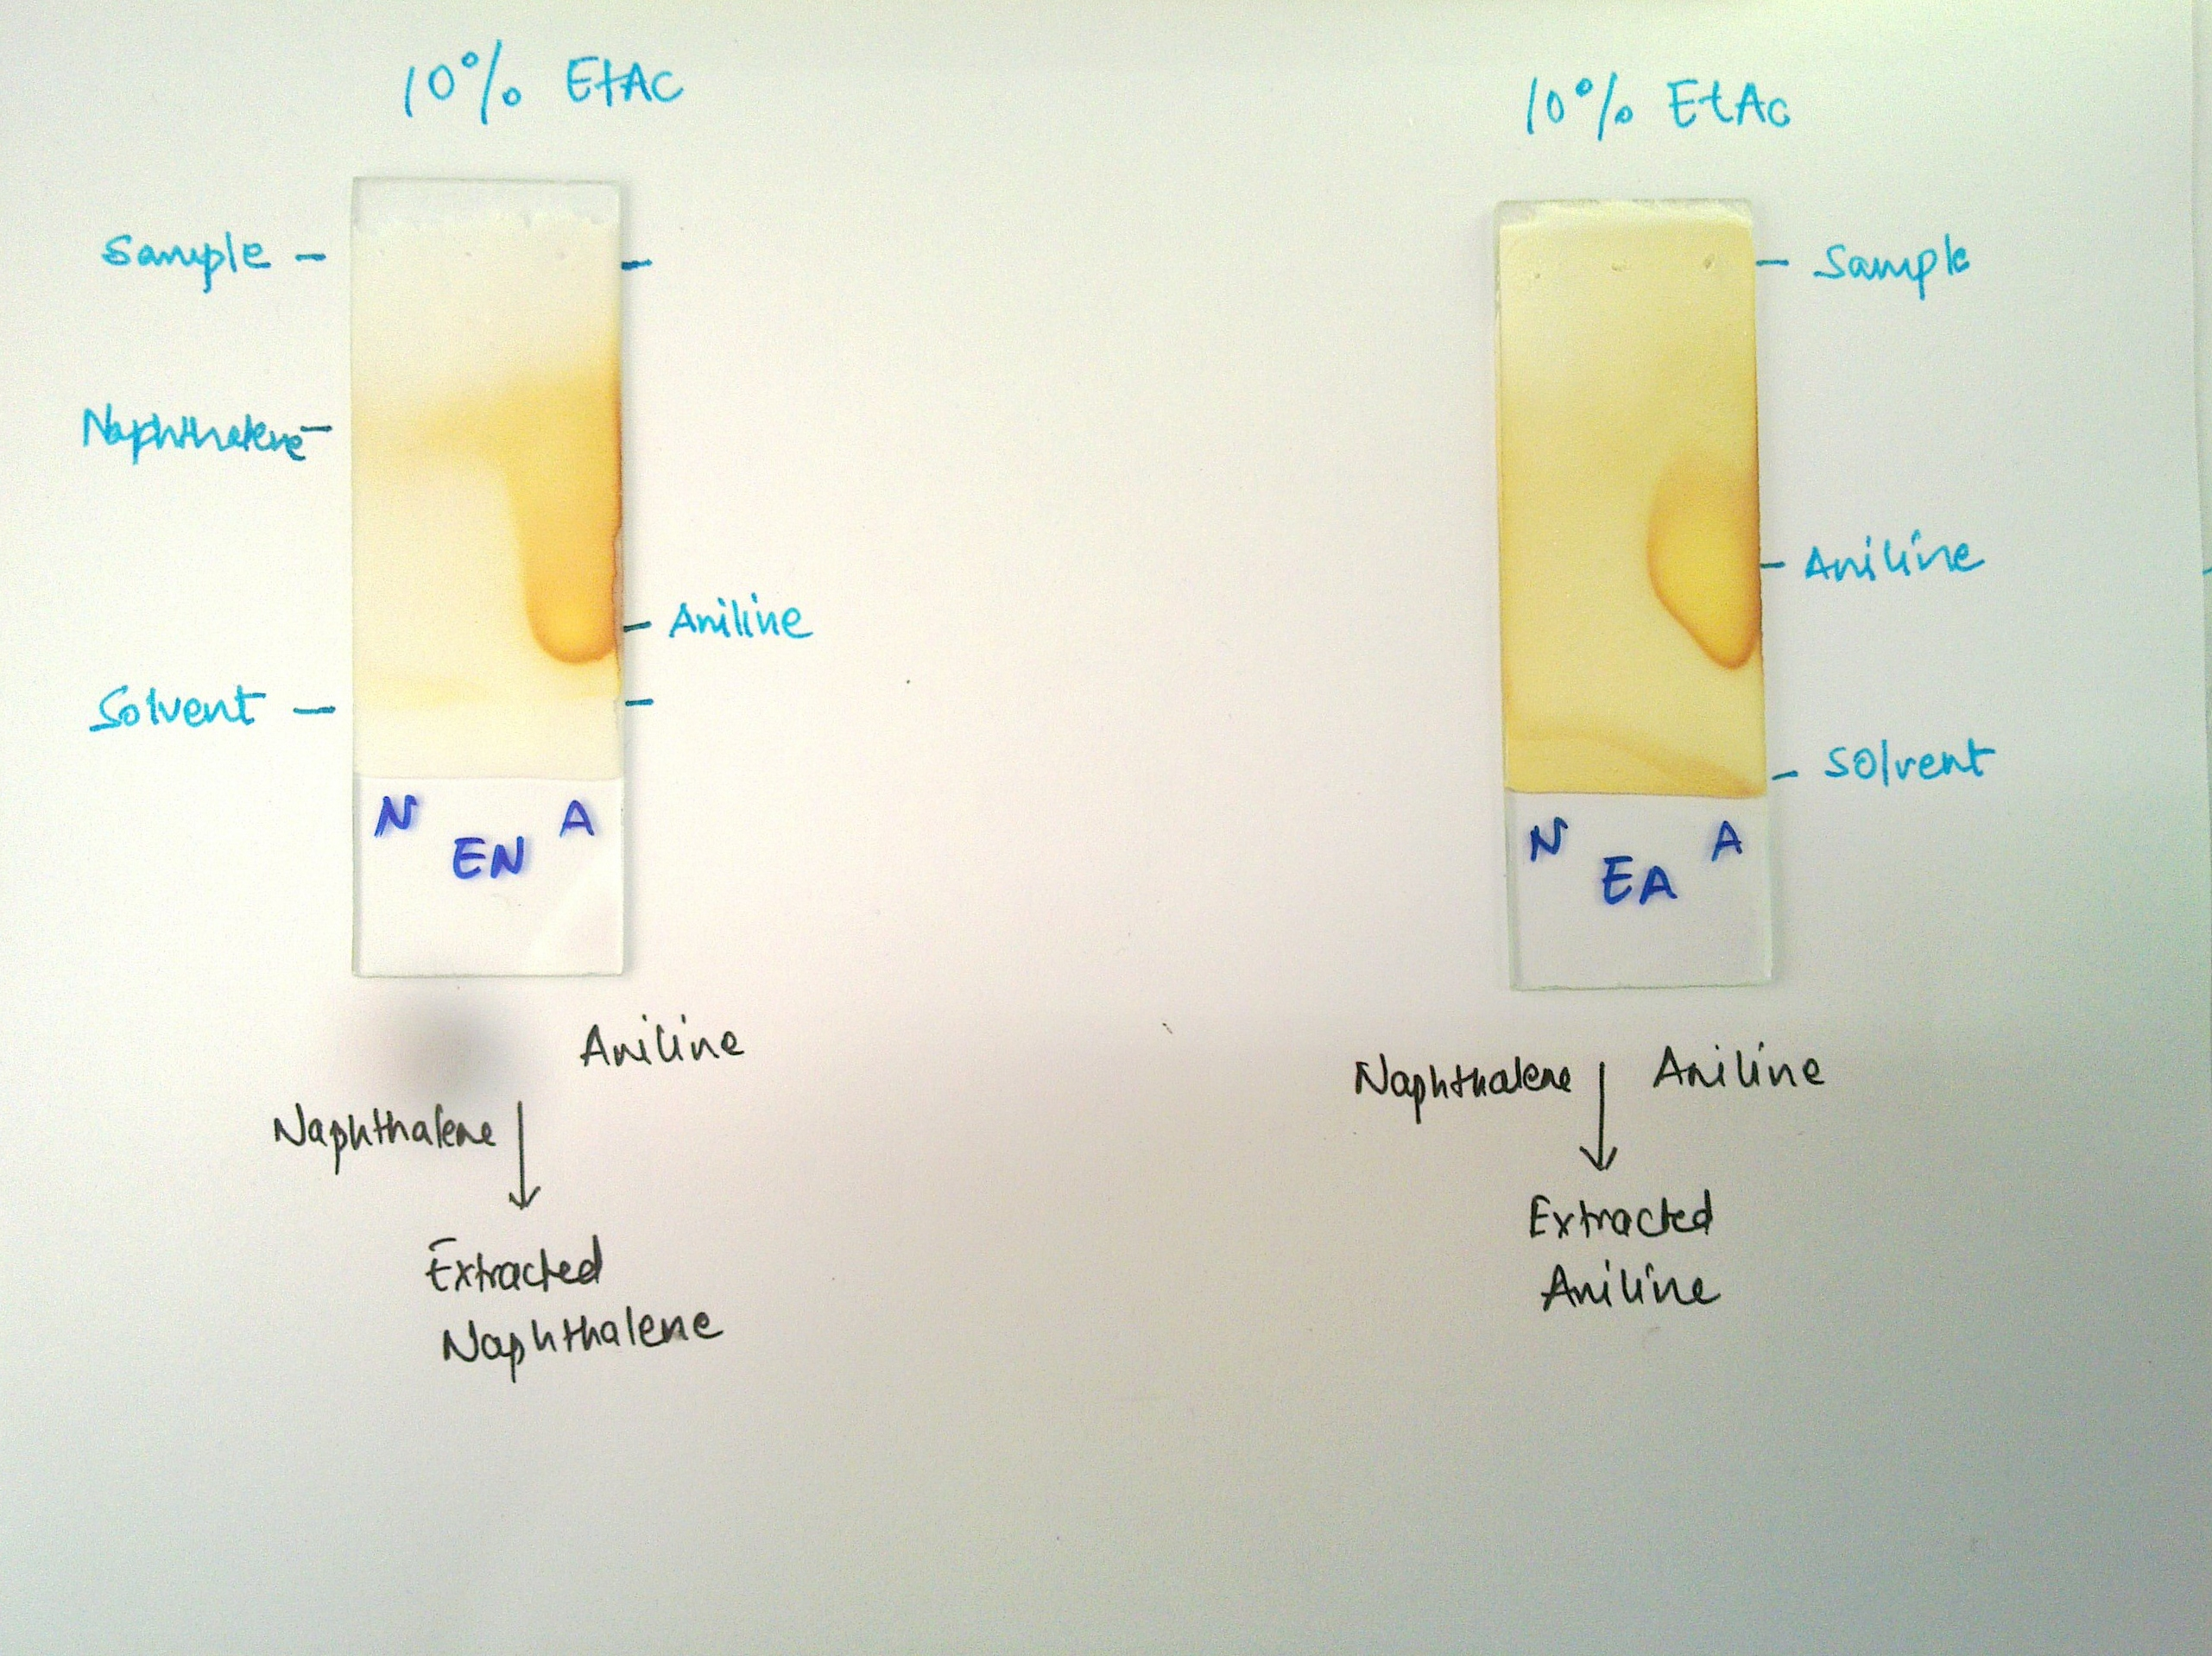
\includegraphics[width=1.0\linewidth]{gfx/e9_tlc}
		\end{center}
	\caption[TLC for Napthalene]{\label{e9_tlc}}
	\end{figure}

	\begin{enumerate}
		\item Naphthalene
		\item Aniline
		\item HCl (catalyst)
		\item Ethanol
		\item Ice
		\item Filter paper
		\item Silica Slurry
		\item $10\%$ Ethyl Acetate in Hexane (for TLC)
	\end{enumerate}

	% \begin{figure}[bth]
	% 	\begin{center}
	% 		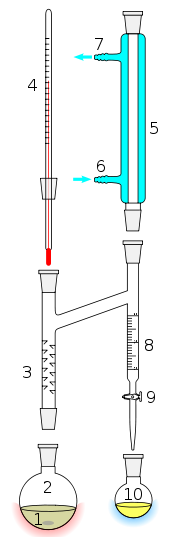
\includegraphics[width=0.4\linewidth]{gfx/e8_setup}
	% 	\end{center}
	% \caption[2-Naphthol]{\label{e8_setup}}
	% \end{figure}

\section{Theory}
	Crystallisation is the process of formation of solid crystals precipitating from a solution.
	\par
	It is an aspect of precipitation obtained through a variability of solubility conditions of the solute in the solvent, as compared to precipitation due to a chemical reaction.
	\par
	Choice of a solvent is very important for crystallisation. For instance, if a compound is polar and the other is non-polar, and we use hexan as the solvent, then the non-polar will get dissolved completely. Upon cooling then, the polar compound will crystallise out while the solution would contain the non-polar solvent. This very phenomenon is used to purify in this experiment.

\section{Procedure}
	\begin{enumerate}
		\item About 1g of a mixture of Napthalene and Aniline were added to 3-5 mL of rectified spirit.
		\item This solution was boiled to dissolve both the substances. Naphthalene however remains dissolved only at high tempreatures (compared to that required for dissolution of aniline of a comparable concentration)
		\item The solution was then cooled and filtered
		\item The filtrate was washed with ice cold ethanol to remove any traces of soluble impurities sticking to the crystal.
		\item The crystals were separated and the TLC checked.
	\end{enumerate}

\section{Observations and Results}
	Naphthalene crystals were obtained and their purity confirmed by TLC as is given in \autoref{e9_tlc}.	

\section{Precaution}
	\begin{enumerate}
		\item The heating was done indirectly to avoid setting Ethanol to fire.
	\end{enumerate}

	
\section{Acknowledgements}
I thank Dr. R Vijaya Anand for his guidance during the experiment. I also acknowledge the contribution of my lab partners, Srijit, Prashansa and Vivek for performance of the same. I also thank our PhD guide for demonstrating the experiment and her assistance in general, with performance of the same.

	% \clearpage
	% \begin{figure}[bth]
	% 	\begin{center}
	% 		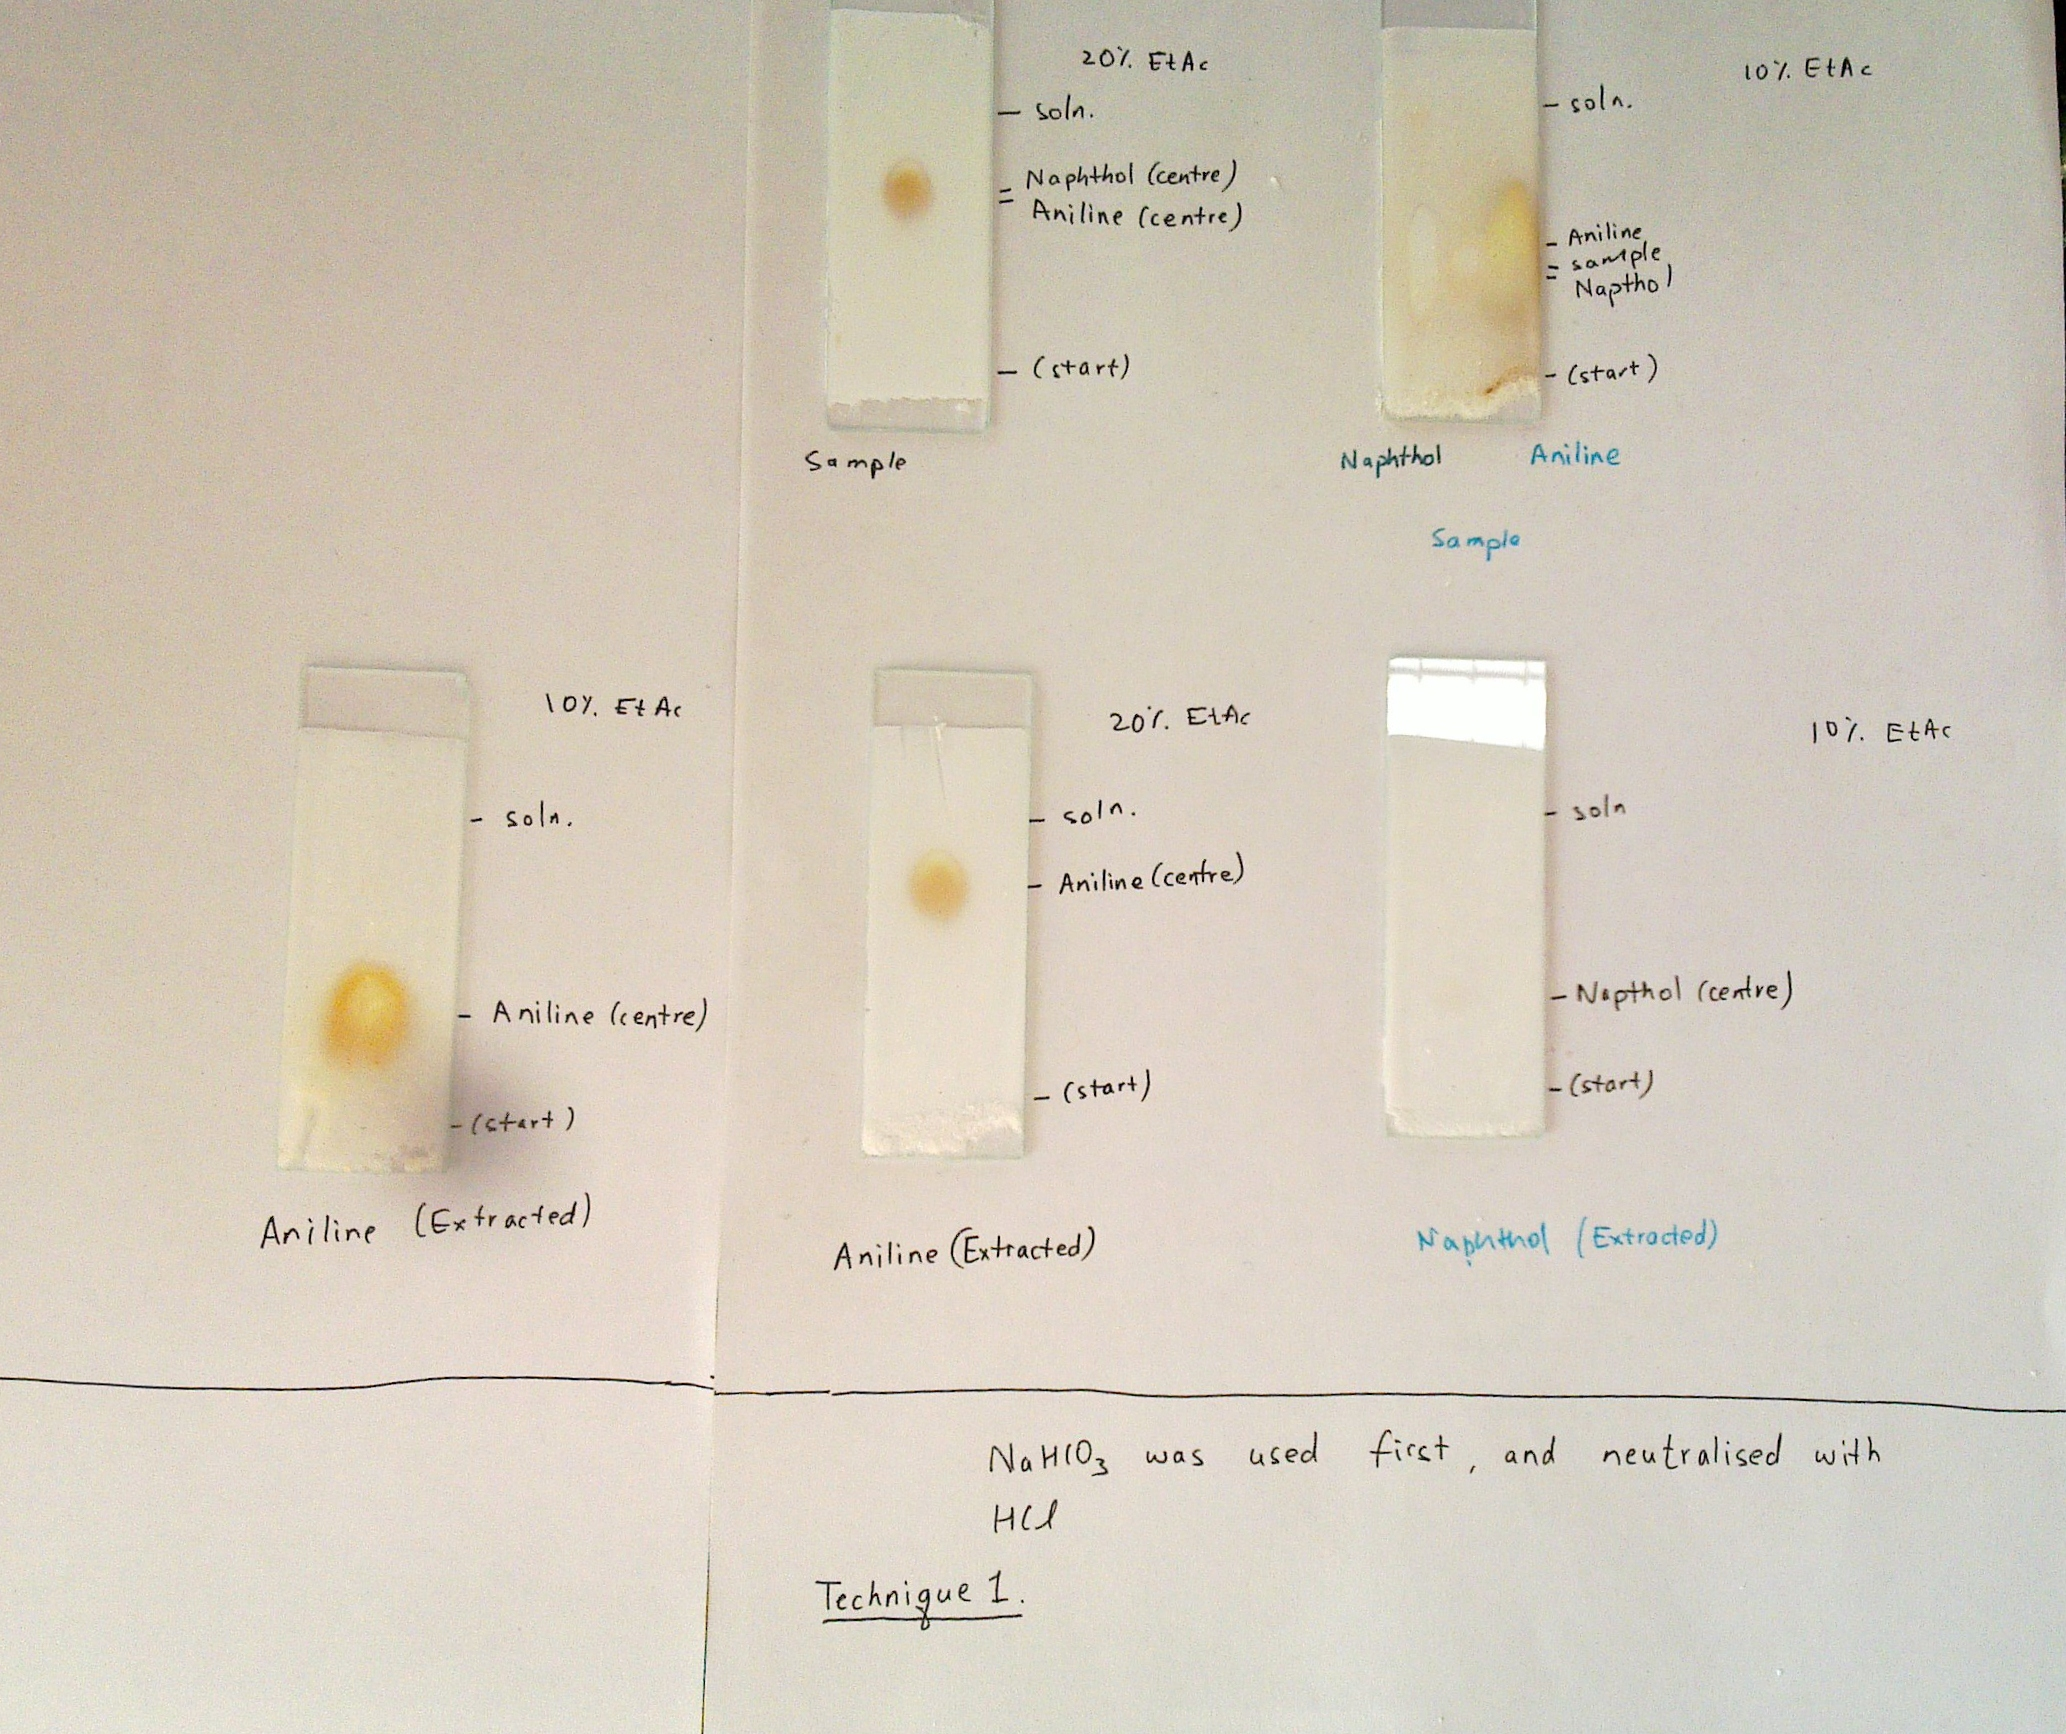
\includegraphics[width=1.5\linewidth]{gfx/e5_1}
	% 	\end{center}
	% \caption[TLCs Set 1]{\label{e5_1}}
	% \end{figure}

	% \begin{figure}[bth]
	% 	\begin{center}
	% 		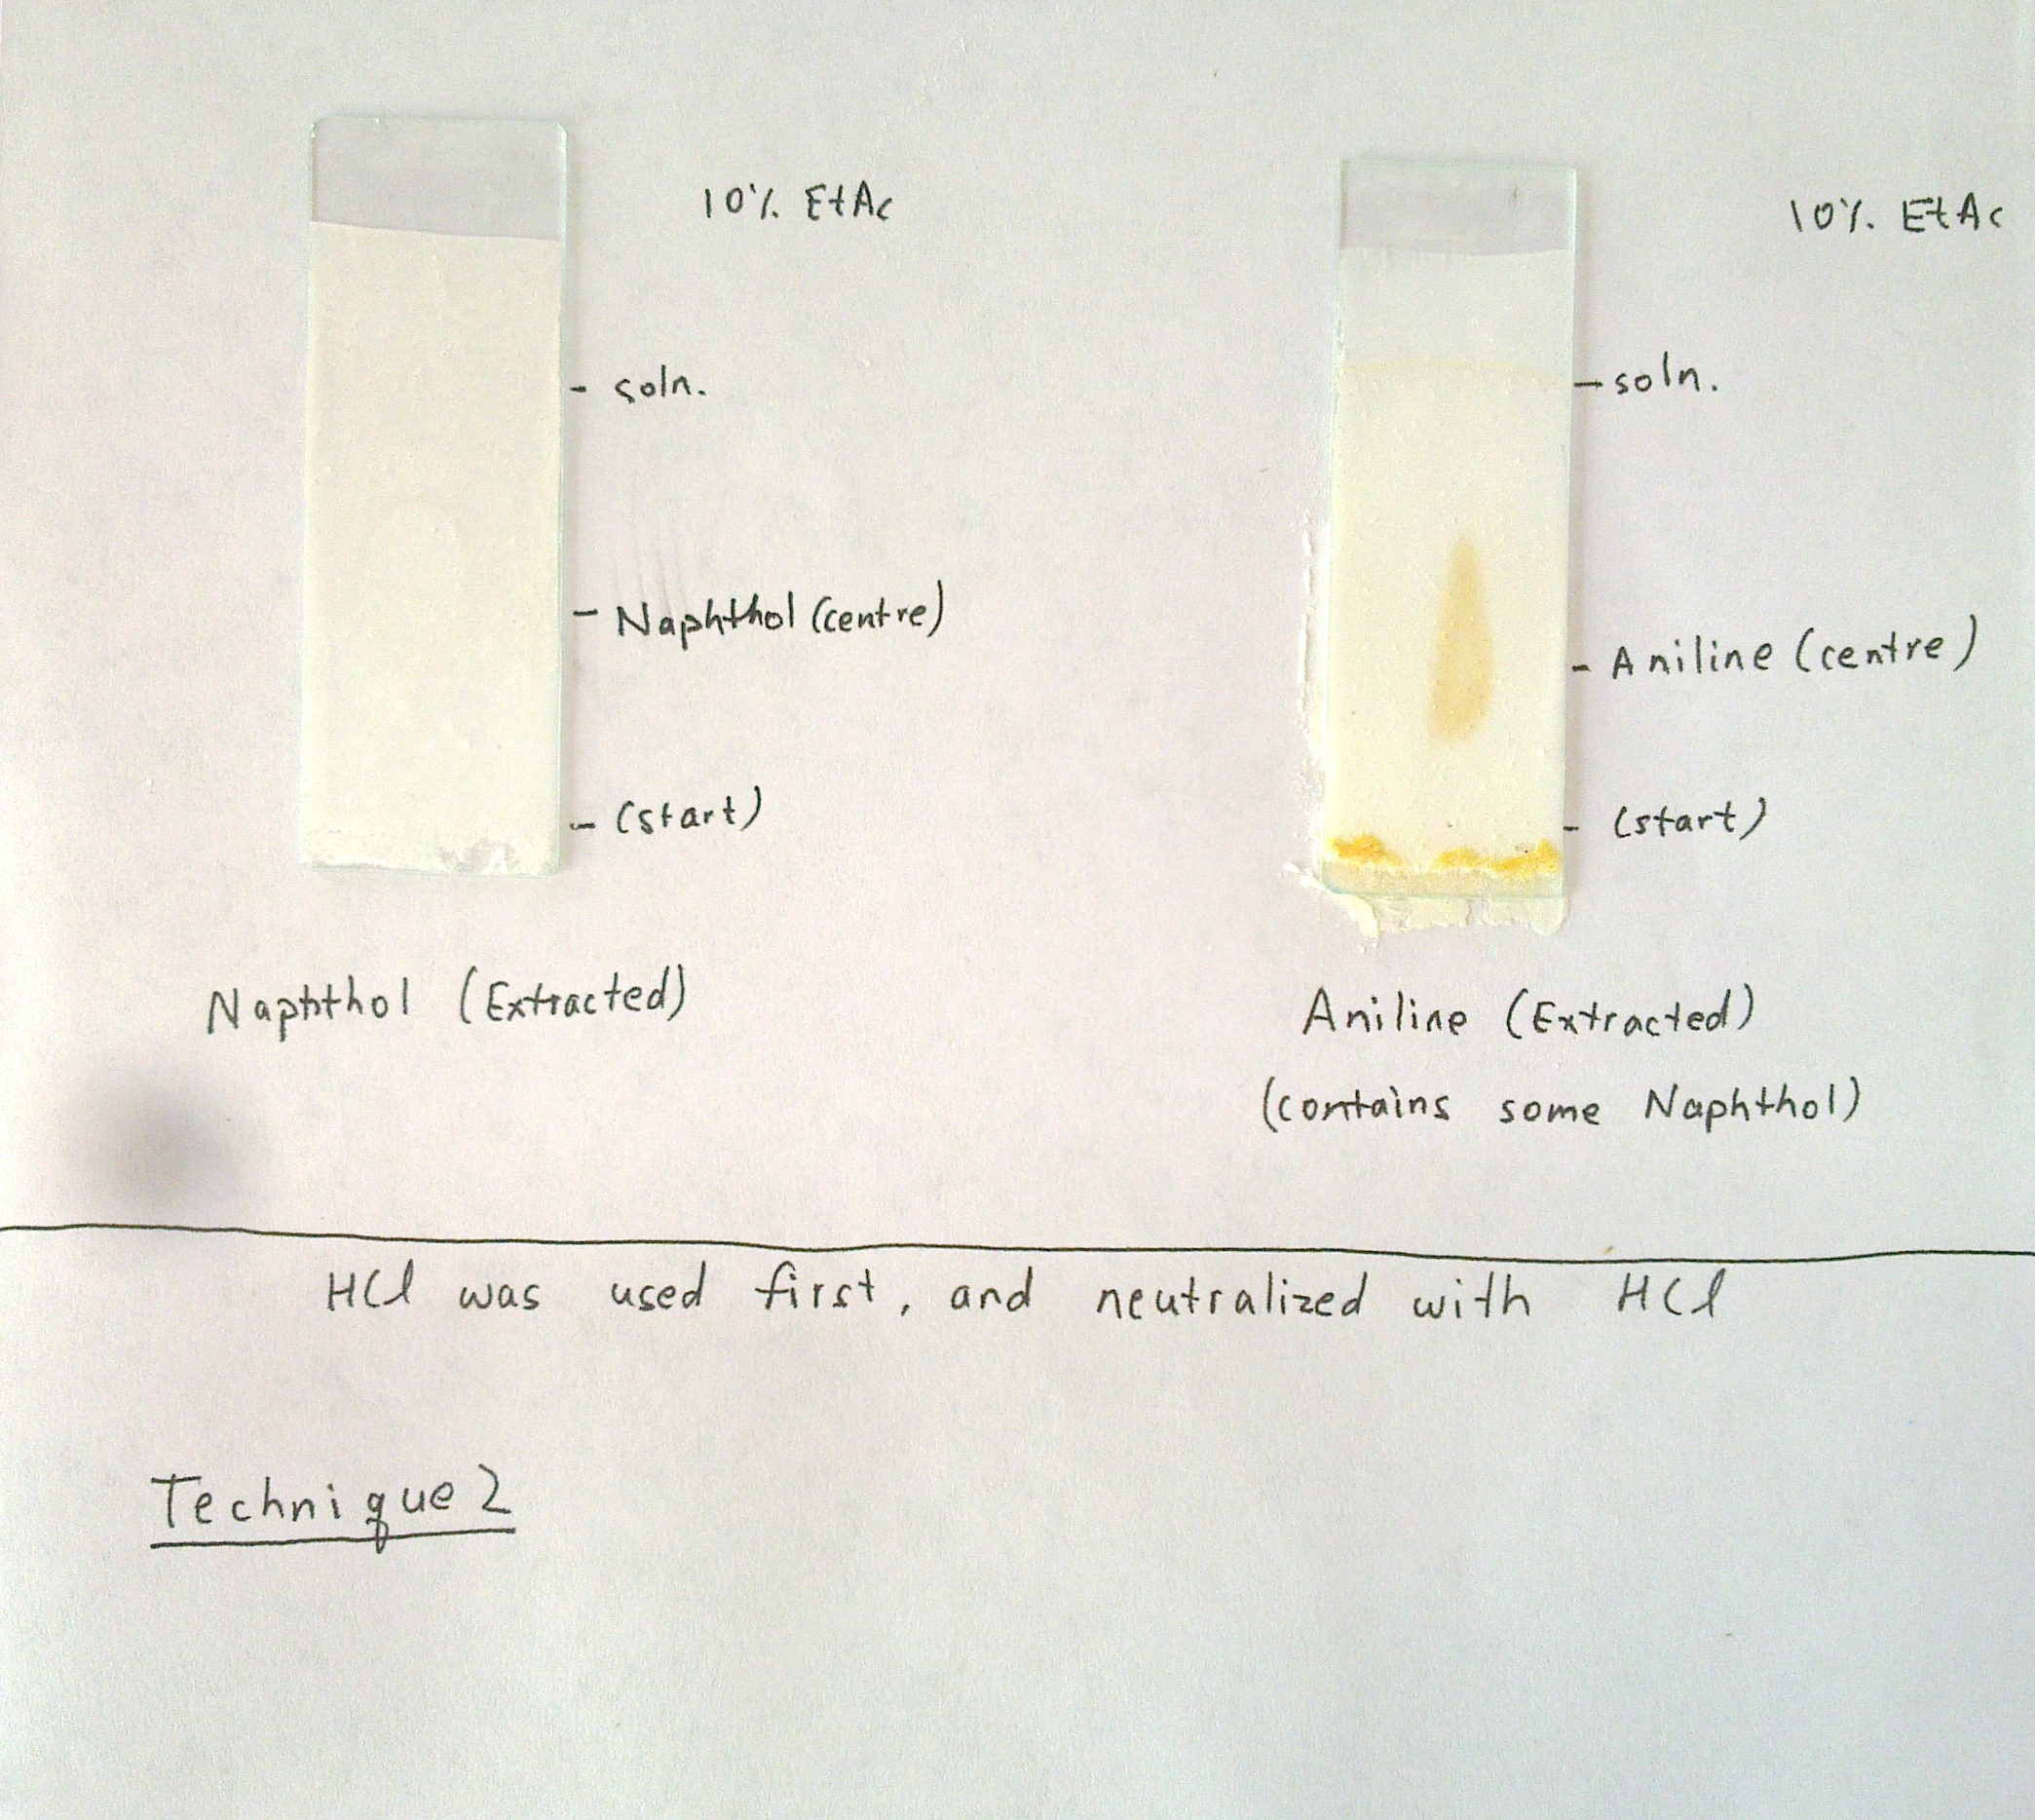
\includegraphics[width=1.0\linewidth]{gfx/e5_2}
	% 	\end{center}
	% \caption[TLCs Set 2]{\label{e5_2}}
	% \end{figure}